% CVPR 2027 paper; cvpr.sty matches the official CVPR2027-v1 ZIP linked by the author guide.
% Follow-up to the ISBI 2027 submission (paper/isbi2027/, do not edit).
% Writing rules: one sentence per line, English, no em dashes, subject first, one claim per sentence,
% define every term before its first use, every number cites its results file.

\documentclass[10pt,twocolumn,letterpaper]{article}
\usepackage[T1]{fontenc}

%%%%%%%%% PAPER TYPE  - PLEASE UPDATE FOR FINAL VERSION
% \usepackage{cvpr}              % To produce the CAMERA-READY version
\usepackage[review]{cvpr}      % To produce the REVIEW version
% \usepackage[pagenumbers]{cvpr} % To force page numbers, e.g. for an arXiv version

% Import additional packages in the preamble file, before hyperref
% Shared packages only; no font, margin, or spacing overrides.
\usepackage{amssymb,graphicx}

\usepackage{booktabs}
\usepackage{multirow}
\usepackage{amsmath}
\usepackage{multicol}

% Status markers for every reported number (see sec/3_methods.tex, "Result status").
\newcommand{\statusfinal}{\textsuperscript{F}}
\newcommand{\statuspre}{\textsuperscript{P}}
\newcommand{\notrun}{\textit{not run}}
% Points to the results file a table was read from.
\newcommand{\src}[1]{\texttt{\detokenize{#1}}}

\definecolor{cvprblue}{rgb}{0.21,0.49,0.74}
\usepackage[pagebackref,breaklinks,colorlinks,allcolors=cvprblue]{hyperref}

\def\confName{CVPR}
\def\confYear{2027}

%%%%%%%%% TITLE - PLEASE UPDATE
\title{Identity Ladder: Population References for\\
Inpainting and Conditional Generation}

%%%%%%%%% AUTHORS - anonymous in review mode
\author{Anonymous \confName~submission}

\begin{document}
% Title and abstract span the page width; the abstract is set in two columns inside that block (Kate, 2026-11-10).
\twocolumn[{%
\renewcommand\twocolumn[1][]{#1}%
\maketitle
\renewenvironment{abstract}{\begin{center}{\large\bfseries Abstract}\end{center}\vspace{-1ex}%
  \begin{multicols}{2}\itshape\small}{\end{multicols}\vspace{1.5ex}}%
\begin{abstract}
\TODO{Abstract after Methods and Results are agreed.}
\end{abstract}
%
}]
\begin{figure*}[t]
\centering
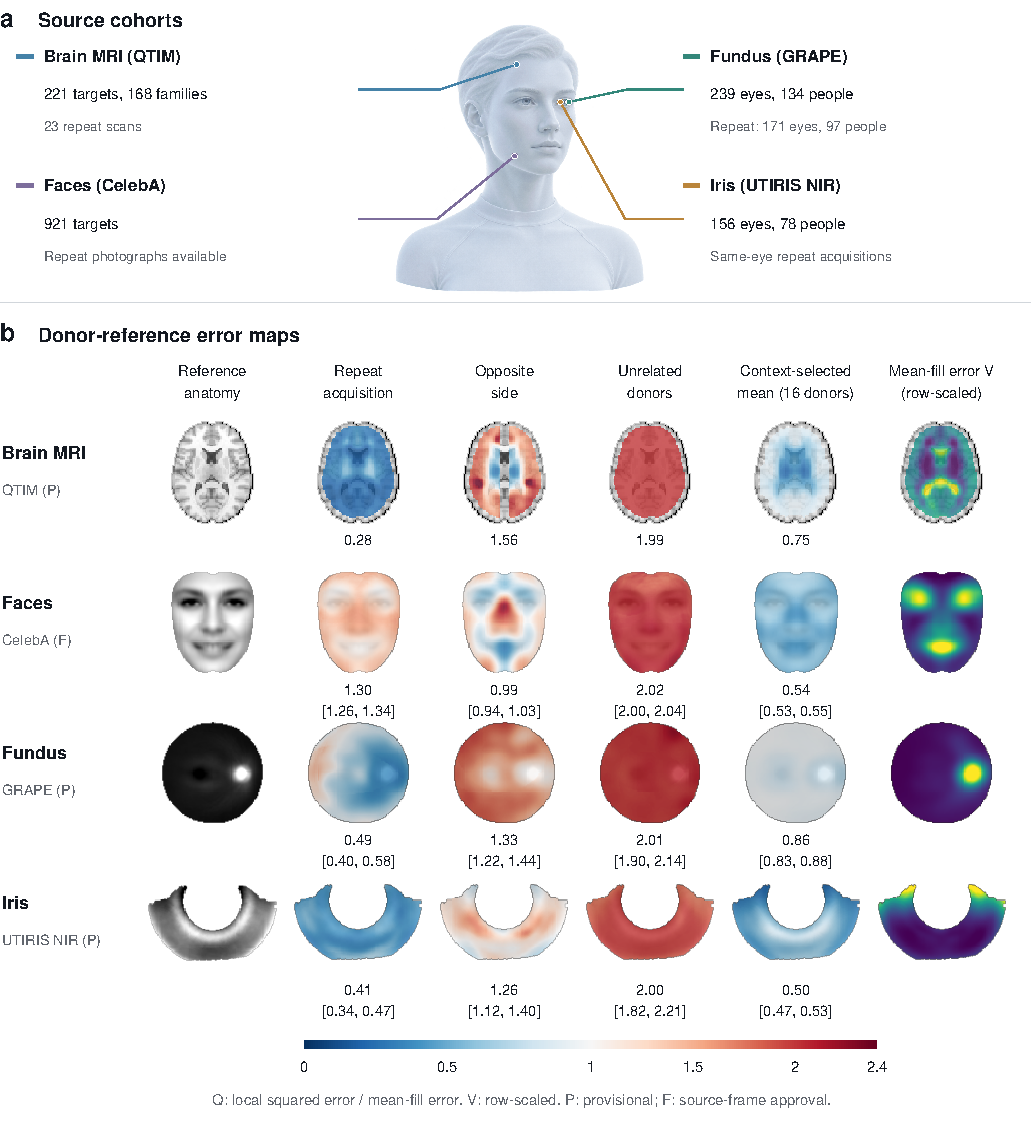
\includegraphics[width=\textwidth]{fig/identity_ladder_provenance_v2.pdf}
\caption{\textbf{Source cohorts and population-reference error maps.}
\textbf{a,} Cohorts and counts; eligibility varies by comparison, with GRAPE repeat coverage shown separately.
\textbf{b,} Observed donor controls: local squared-error ratios against an independent mean fill ($Q=1$).
References are population means or an independent MRI template.
Pooled numbers differ from the anchored window-level tables; recorded intervals appear where available.
Context-selected means use 16 donors; V is row-scaled.
Rows use modality-specific display sizes.
The pale MRI outline and shared crop are display-only; brain windows are Gaussian.
Fundus uses GRAPE P8 and iris uses P2.
F denotes source-frame approval; P denotes provisional evidence.
The bust is decorative and synthetic; secondary datasets and display provenance remain in the supplement.}
\label{fig:atlas}
\end{figure*}
\section{Introduction}
\label{sec:intro}
\TODO{Introduction. Position against CARE, OCT LMSB, Brain-ID and restoration theory; every citation through bib-verify.}

\section{Related work}
\label{sec:related}
\paragraph{Reconstruction and perceptual quality.}
The perception--distortion tradeoff separates reference distortion from distributional perceptual quality~\cite{blau2018}.
Learned Perceptual Image Patch Similarity (LPIPS) evaluates aspects of visual similarity that pixel distances miss~\cite{zhang2018lpips}.
Neither objective alone defines whether the retained detail belongs to the target person.
Our audit adds controlled person-, organ-, and acquisition-level comparisons to this distinction.
Structural similarity (SSIM) supplies a local reference comparison~\cite{wang2004}, but its interpretation still depends on the anatomical and acquisition changes represented by a pair.

\paragraph{Anatomical completeness and harmonization.}
CARE evaluates sparse-view CT reconstruction using anatomy-aware measurements of large and small organs, intestines, and vessels~\cite{care2025}.
Its objective is structural completeness rather than validation of a donor-based identity scale.
LMSB addresses anatomical changes in OCT harmonization by learning an anatomy-guided latent metric before distribution matching~\cite{lmsb2025}.
It demonstrates why Euclidean proximity in appearance need not coincide with anatomical consistency.
Our contribution is an evaluation design around such interpretations, not an empirical comparison against either reconstruction or harmonization system.

\paragraph{Anatomical representations and biometric units.}
Brain-ID learns contrast-agnostic anatomical features from synthetic inputs and evaluates robustness and downstream brain-imaging tasks~\cite{brainid2024}.
Those results motivate acquisition controls, but a Brain-ID distance has not been completed in this study.
Iris recognition illustrates a complementary distinction: a person has two eyes, and person membership does not make their iris textures one biometric instance~\cite{daugman2004,daugman2001}.
The relevant identity unit must therefore be specified before an anatomical similarity result is interpreted.
ArcFace supplies an identity-oriented face representation~\cite{arcface2022}; our local-donor analysis distinguishes that whole-image reference from the window-level reconstruction distance.

\paragraph{Task-specific metric validation.}
Metrics Reloaded emphasizes matching validation measures to the task and data~\cite{metrics2024}.
We operationalize that principle through separate controls for attenuation, incorrect detail, bilateral correspondence, and acquisition.
A successful check on one axis does not establish success on the others.

\section{Methods}
\label{sec:methods}

% One subsection per modality: data and rungs, protocol (file + amendment), preprocessing and alignment, metrics.
% Inventory approved by Kate before prose is drafted.

\subsection{The donor ladder and the unit}
\label{sec:ladder}
\TODO{Rungs, unit V, ratio = sum of errors / sum of V, bootstrap over families. Source: docs/PROTOCOL\_donor\_ladder\_general.md sections 1--6.}

\subsection{Result status}
\label{sec:status}
\TODO{Final (F), provisional pre-QC (P), not run. Missing is never zero.}

\subsection{Brain MRI (QTIM)}
\label{sec:m-brain}
\TODO{docs/PROTOCOL\_donor\_ladder\_brain.md, Amendments 1--9.}

\subsection{Fundus photographs (PAPILA, GRAPE)}
\label{sec:m-fundus}
\TODO{docs/PROTOCOL\_donor\_ladder\_fundus.md; docs/PROTOCOL\_donor\_ladder\_general.md section 9, Amendments 9.1--9.4.}

\subsection{Face photographs (CelebA, IMDb-WIKI)}
\label{sec:m-face}
\TODO{docs/PROTOCOL\_donor\_ladder\_face.md (not yet committed), Amendments 1--8.}

\subsection{Iris images (UTIRIS, UPOL)}
\label{sec:m-iris}
\TODO{No pixel donor ladder yet; iris codes and calibration only.}

\subsection{Synthetic simulations}
\label{sec:m-sim}
\TODO{src/theory\_sim.py, toy ladder, population null, label ladder.}

\section{Results}
\label{sec:results}
% Every table cites its results file with \src{...} and marks each value F, P or not run.

\subsection{An inpainting-evaluator case study}
Saved synthetic probes of BraTS \texttt{inpainting} 0.0.12 identify a two-spatial-axis SSIM convention and PSNR clipping that breaks exact rank equivalence with MSE.
They motivate an explicit implementation contract, not a claim of independent anatomical sensitivity.
The supplement retains both dependency-version records and all numerical probes; no generator or organizer-server validation is implied.
% Sources: results/brats_panel_checks_tm1.1.2.json and brats_panel_checks_tm1.9.0.json.

\subsection{Brain MRI (QTIM)}
\label{sec:r-brain}
All brain-panel findings in this section are provisional.
Table~\ref{tab:brain} reports the saved random-region, both-hemisphere profile, with source two-way intervals.
The MSE position of the dataset mean is below the mirror position, while the corresponding ordering changes under TM-like distance.
The difference is an observed metric profile under the recorded alignment, not evidence that a population mean preserves more of a person's anatomy.

The tests also distinguish separate requirements.
MSE establishes that the repeat is better than the dataset mean, incorrect detail, and noise in the recorded directional tests.
It does not establish that the repeat is better than its attenuated version.
The attenuated-repeat MSE position is $-0.014$ with interval $[-0.028,-0.004]$\statuspre, where the original repeat is the zero anchor.
For the repeat-tolerance lDDT-like measure, the corresponding position is $-0.084$ with interval $[-0.108,-0.065]$\statuspre.
These findings show a possible attenuation preference while leaving the registration gate unresolved.
They do not make failure of T2 a general theorem about those metrics.
% Numerical source: donor_ladder_brain_metrics.json, views/random_patches/LR/ladder_R.

\begin{table*}[t]
\centering
\caption{\textbf{Provisional brain audit profile.} $R_{\rm rep}$: repeat zero and mean of the recorded unrelated donors one; lower is closer.
Cells contain means and source 95\% intervals, with family and position resampling.
Non-repeat rows involve 221 targets from 168 families; the repeat anchor involves 23 targets.
Residual correlation at the exact dataset mean is undefined.
Source: \src{results/donor_ladder_brain_metrics.json}.}
\label{tab:brain}
\small
\begin{tabular}{@{}lcccc@{}}
\toprule
Metric & Dataset mean & Mirror & Incorrect detail & Noise \\
\midrule
MSE & \shortstack{0.413\statuspre\\{\scriptsize [0.367, 0.443]}} & \shortstack{0.717\statuspre\\{\scriptsize [0.622, 0.792]}} & \shortstack{1.006\statuspre\\{\scriptsize [0.992, 1.020]}} & \shortstack{0.921\statuspre\\{\scriptsize [0.893, 0.944]}} \\
SSIM & \shortstack{0.738\statuspre\\{\scriptsize [0.680, 0.784]}} & \shortstack{0.823\statuspre\\{\scriptsize [0.755, 0.873]}} & \shortstack{1.023\statuspre\\{\scriptsize [1.014, 1.036]}} & \shortstack{1.132\statuspre\\{\scriptsize [1.088, 1.194]}} \\
Residual correlation & \textit{undefined} & \shortstack{0.752\statuspre\\{\scriptsize [0.688, 0.808]}} & \shortstack{1.003\statuspre\\{\scriptsize [0.996, 1.009]}} & \shortstack{1.003\statuspre\\{\scriptsize [1.000, 1.006]}} \\
TM-like & \shortstack{0.723\statuspre\\{\scriptsize [0.642, 0.778]}} & \shortstack{0.667\statuspre\\{\scriptsize [0.530, 0.761]}} & \shortstack{0.997\statuspre\\{\scriptsize [0.987, 1.007]}} & \shortstack{1.075\statuspre\\{\scriptsize [1.041, 1.121]}} \\
lDDT-like, repeat tolerance & \shortstack{0.355\statuspre\\{\scriptsize [0.254, 0.430]}} & \shortstack{0.890\statuspre\\{\scriptsize [0.843, 0.925]}} & \shortstack{1.050\statuspre\\{\scriptsize [1.030, 1.080]}} & \shortstack{2.073\statuspre\\{\scriptsize [1.924, 2.273]}} \\
\bottomrule

\end{tabular}
\end{table*}

HACA3+ stage 1 provides a separate contrast sensitivity, not a completed identity endpoint.
Across its 23 paired scans, mean absolute deep-region session shift changes from $0.121$ to $0.016$ standardized intensity units\statuspre.
The parietal counterpart changes from $0.059$ to $0.033$\statuspre.
The source records a pending visual verdict, and neither measurement establishes preservation of subject-specific detail.
% Numerical source: donor_ladder_brain_haca3_stage1.json, session_shift_z.

\subsection{Fundus photographs (PAPILA, GRAPE)}
\label{sec:r-fundus}
The frozen bilateral-branch aggregate supplies the P8/P9 frame-only profile in Table~\ref{tab:fundus}.
GRAPE has 239 target-eye units from 134 people in the stranger comparison; the repeat comparison has 171 units from 97 people\statuspre.
PAPILA has 488 target eyes from 244 people and no other-visit rung\statuspre.
The dataset mean is closer than the fellow eye under squared error in both saved summaries.
The context-selected mean of look-alikes can outperform the unconditional mean in this representation.
These findings are provisional and do not establish the identity of the inferred detail.

\begin{table*}[t]
\centering
\caption{\textbf{Provisional frame-only fundus profile.}
Mean-relative squared-error ratio $Q$, with source person-bootstrap intervals; lower is closer.
These P8/P9 map-compatible summaries differ from the older P7 support and from the window-level metric panel.
PAPILA has no repeat observation.
Source: \src{results/donor_ladder_2d_facefmt.json} at the frozen bilateral snapshot, copied without change into the paper inputs.}
\label{tab:fundus}
\small
\begin{tabular}{@{}lcccc@{}}
\toprule
Dataset & Repeat & Fellow eye & Context mean & Stranger \\
\midrule
GRAPE P8 & \shortstack{0.489\statuspre\\{\scriptsize [0.404, 0.585]}} & \shortstack{1.330\statuspre\\{\scriptsize [1.224, 1.437]}} & \shortstack{0.856\statuspre\\{\scriptsize [0.832, 0.880]}} & \shortstack{2.012\statuspre\\{\scriptsize [1.897, 2.140]}} \\
PAPILA P9 & \textit{unavailable} & \shortstack{1.467\statuspre\\{\scriptsize [1.422, 1.512]}} & \shortstack{0.935\statuspre\\{\scriptsize [0.914, 0.955]}} & \shortstack{1.992\statuspre\\{\scriptsize [1.941, 2.049]}} \\
\bottomrule

\end{tabular}
\end{table*}

The Gaussian maps in Figure~\ref{fig:atlas} retain these preprocessing labels.
High split-half correlation cannot establish anatomical validity if a shared preprocessing artifact is reproducible too.
The completed v1 metric registry and the running newer extension remain separate.
Superseded support-sensitive block searches supply no primary result.

\subsection{Face photographs (CelebA, IMDb-WIKI)}
\label{sec:r-face}
Table~\ref{tab:face} reports the available v6f tier-1 profiles on the self-anchored scale.
The repeat photograph has substantial pixel error despite preserving person membership.
The dataset mean is closer than the repeat under MSE in both datasets, while a local context-selected donor is closer still.
That pixel preference does not identify the donor as the target person.

For CelebA, the selected donor's local MSE position is $0.399$\statusfinal, while its whole-image ArcFace donor-reference position is $0.983$\statusfinal.
The corresponding IMDb-WIKI values are $0.397$ and $0.984$\statusfinal.
These are different measurements at different spatial scopes.
Their disagreement shows that local photometric matching can select a donor whose global identity representation remains near the unrelated reference.
It does not measure identity retention by a completed composite reconstruction, and no ArcFace value is assigned to an unembedded mean.

\begin{table*}[t]
\centering
\caption{\textbf{Face metric and donor-identity profiles.} Recorded $R_{\rm self}$ point estimates; target self zero, mean of unrelated donors one.
The source retains family/position bootstrap intervals; full records accompany the preparation manifest.
The approved frame has 921 CelebA targets and 678 IMDb-WIKI targets, respectively clustered into 921 and 453 units.
ArcFace compares whole target and donor images; the pixel metrics compare local windows.
Source: \src{results/face_ladder_metrics.json}.}
\label{tab:face}
\small
\begin{tabular}{@{}llcccc@{}}
\toprule
Dataset & Metric & Retest & Bilateral & Dataset mean & Context donor \\
\midrule
CelebA & MSE & 0.640\statusfinal & 0.475\statusfinal & 0.499\statusfinal & 0.399\statusfinal \\
CelebA & SSIM & 0.828\statusfinal & 0.693\statusfinal & 0.844\statusfinal & 0.726\statusfinal \\
CelebA & ArcFace donor reference & 0.354\statusfinal & \textit{unavailable} & \textit{unavailable} & 0.983\statusfinal \\
IMDb-WIKI & MSE & 0.690\statusfinal & 0.529\statusfinal & 0.498\statusfinal & 0.397\statusfinal \\
IMDb-WIKI & SSIM & 0.856\statusfinal & 0.739\statusfinal & 0.859\statusfinal & 0.743\statusfinal \\
IMDb-WIKI & ArcFace donor reference & 0.396\statusfinal & \textit{unavailable} & \textit{unavailable} & 0.984\statusfinal \\
\bottomrule

\end{tabular}
\end{table*}

\subsection{Iris images (UTIRIS, UPOL)}
\label{sec:r-iris}
The current P2 strip panel contains 156 target eyes from 78 people for UTIRIS NIR.
The secondary UTIRIS VIS and UPOL panels contain 158 eyes from 79 people and 128 eyes from 64 people, respectively\statuspre.
The VIS repeat endpoint has one fewer eligible eye, which is retained as endpoint-specific coverage rather than silently changing every comparison.
Table~\ref{tab:iris} reports mean-relative squared error on the support defined for each condition.
The repeated eye is closer than the fellow eye in all three saved summaries, and a context-selected unrelated donor can fall between them.
These are pixel-space relationships; they are not an iris biometric verification result.

\begin{table*}[t]
\centering
\caption{\textbf{Provisional P2 iris donor ladder.} Squared-error ratio $Q$ against an independent dataset mean evaluated on the same support; lower is closer.
The mean anchor is one by construction; an independent equal-variance stranger has theoretical expectation near two.
Intervals use person bootstrap.
Target-eye/person counts are 156/78, 158/79, and 128/64; the VIS repeat endpoint uses 157 eyes.
Source: \src{results/iris_ladder_metrics.json}, results block.}
\label{tab:iris}
\small
\begin{tabular}{@{}lcccc@{}}
\toprule
Dataset & Same-eye repeat & Fellow eye & Context donor & Stranger \\
\midrule
UTIRIS NIR & \shortstack{0.407\statuspre\\{\scriptsize [0.345, 0.475]}} & \shortstack{1.256\statuspre\\{\scriptsize [1.123, 1.395]}} & \shortstack{0.599\statuspre\\{\scriptsize [0.540, 0.660]}} & \shortstack{2.001\statuspre\\{\scriptsize [1.816, 2.207]}} \\
UTIRIS VIS & \shortstack{0.569\statuspre\\{\scriptsize [0.503, 0.640]}} & \shortstack{1.293\statuspre\\{\scriptsize [1.211, 1.375]}} & \shortstack{0.861\statuspre\\{\scriptsize [0.826, 0.898]}} & \shortstack{2.018\statuspre\\{\scriptsize [1.884, 2.176]}} \\
UPOL & \shortstack{0.177\statuspre\\{\scriptsize [0.154, 0.200]}} & \shortstack{1.118\statuspre\\{\scriptsize [1.037, 1.198]}} & \shortstack{0.841\statuspre\\{\scriptsize [0.798, 0.882]}} & \shortstack{2.138\statuspre\\{\scriptsize [2.007, 2.281]}} \\
\bottomrule

\end{tabular}
\end{table*}

The source retains distinct $R_{\rm self}$ and $R_{\rm rep}$ values, window-level controls, and the directional tests.
It also records a lid-shadow mask review limitation.
The newer full P3 run is absent from this aggregate snapshot.
Consequently, its LPIPS, Betti-matching, FID, and FWD outcomes are not numerically reconstructed from P2 or from old iris-code results.

\subsection{Synthetic simulations}
\label{sec:r-sim}
The saved synthetic experiments isolate a complementary ambiguity.
On the known-target attenuation path, an image can keep a high unrelated-reference rank while its residual amplitude falls.
An amplitude-matched incorrect residual shows why distance from the mean alone is insufficient.
Synthetic pupil dilation holds latent eye parameters fixed while changing appearance, exposing the opposite failure direction.
These controls explain mechanisms, but they do not establish how often the same effect occurs in measured anatomy.
The synthetic label experiments additionally depend on the anatomical prior and segmentation construction.
Their conditional findings do not establish a universal Dice or topology result.

\section{From reference audits to model audits}
\label{sec:synthesis}
The existing experiments characterize reference candidates and metric behavior.
Table~\ref{tab:decision} separates that evidence from the proposed audit of conditional generation across populations.
Coverage describes what has been investigated, not a percentage of a model-evaluation problem solved.

\paragraph{What the references establish.}
Means, attenuation, incorrect residuals, and repeats expose different interpretations of a similarity score.
Symmetry supplies a comparison condition rather than an identity label: a face reflection shares capture conditions, a fellow iris changes the biometric instance, and hemispheres require correspondence.
Cross-anatomy observations stress these interpretations without establishing a universal ordering or transfer to every inpainting task.

\paragraph{How model behavior could be tested.}
For a fixed context and mask, generated outputs can be compared with the same ladder controls using Eq.~\ref{eq:population-audit}.
Repeating this comparison within target strata could reveal whether a model's scores approach global or matched means, retain target-aligned variation, or respond to acquisition differently between groups.
The context must support the claimed detail: a conditional mean can be a legitimate prediction when the withheld content is ambiguous.
Residual correlation misses positive amplitude shrinkage, and stranger calibration supplies no new anatomical information.
The profile therefore retains complementary controls rather than identifying one coordinate with preserved identity.

\paragraph{Population and sampling interpretation.}
Global and matched references answer different questions; group-specific normalization alone can conceal raw gaps or differences in reference variance.
A group contrast characterizes the model--metric system; attribution requires checking reference, acquisition and task-composition effects.
Mask difficulty, location, acquisition, donor-pool size and missing outputs must remain visible in a comparison.
Repeated outputs distinguish variation across targets from variation across seeds for one context; reduced variance alone does not establish mode collapse.
Group gaps require independent-unit uncertainty and an explicit target population, and do not by themselves establish causal discrimination or fairness.
Actual generator outputs, an independent anatomy or task criterion, and held-out validation are needed to test these proposed interpretations.

\paragraph{Limitations and evidence coverage.}
Registration and acquisition remain central confounders in the brain and fundus panels.
Source protocols have advanced beyond some accessible outputs, and preprocessing versions must not be merged by name.
The evidence freeze predates receipt of the base face pipeline and full iris P3 aggregates; integration remains pending.
Lid-shadow information, changing support and selection on usable windows can affect iris comparisons.
The current residual and rank coordinates have not been validated as a fused identity score.
Results at one window size do not establish stability over the latest object-relative size grid.

\paragraph{Ethics and data.}
The manuscript preparation uses existing aggregate outputs and does not read or redistribute participant images or identifiers.
The anatomical map illustrations are population summaries or templates, not individual exemplars.
Iris images and private row tables remain outside the public repository.
The preparation record does not establish the original dataset consent or the institutional basis for each secondary analysis.
Those dataset-specific approval, exemption and consent statements require author confirmation before a submission-ready ethics declaration can be made.

\section{Conclusion}
Identity Ladder supplies population references for interpreting similarity in inpainting and a defined extension to audits of conditional generation.
The measured controls probe responses to detail loss, incorrect detail and acquisition variation; generated-output profiles across target strata remain to be tested.
Broader applications require an appropriate identity unit, conditioning contract and reference population, preserving the distinction between a proposed audit and demonstrated model behavior.

\clearpage
\section*{LLM Usage Statement}
OpenAI Codex assisted with source inspection, manuscript structure and prose, bibliography metadata retrieval, aggregate-to-table preparation code, and build verification.
OpenAI image generation produced the decorative anonymous bust in the provenance illustration; labels, cohort counts and measured heatmaps were assembled separately from recorded sources.
Claude (Anthropic) [CONFIRM model versions] assisted with experimental code, protocols, analyses, figures and text.
No language model created experimental observations or participant images.
The authors remain responsible for checking the scientific claims, evidence status, citations and final text.

{
    \small
    \bibliographystyle{ieeenat_fullname}
    \bibliography{main}
}

% WARNING: do not forget to delete the supplementary pages from your submission
% \section{Scope, provenance, and evidence status}
This supplement documents the source snapshot used to assemble the manuscript.
It does not convert a protocol, a running job, or a workstation report into a completed endpoint.
The preparation script reads public aggregate JSONs, generates tables, copies selected population-summary PDFs, and records input hashes and producing commits in \src{evidence_manifest.json}.
No participant image or per-person result row is read during manuscript assembly.
Figure provenance describes the origin of the saved output; copying it does not independently reproduce the underlying experiment.

The labels \statusfinal\ and \statuspre\ apply to individual results and frames.
A frame can have an approved visual decision while an additional mask change remains unresolved.
An older run can contain valid measurements for its own question while being unsuitable as a replacement for the amended protocol.
The source-level status must therefore accompany every comparison, not just the dataset name.

\subsection{Coverage of the existing research materials}
\begin{table}[htbp]
\centering
\caption{Available cohorts and evidence status.
Units are target people for brain and faces, and target eyes for iris and P8/P9 fundus.
Independent clusters are families or people; the repeat column is endpoint-specific.
Sources: the saved brain, face, iris and frozen fundus metric/map aggregate files recorded in the evidence manifest.}
\label{tab:s-coverage}
\small
\begin{tabular}{@{}lrrll@{}}
\toprule
Dataset & Target units & Clusters & With repeat & Status \\
\midrule
QTIM & 221 & 168 & 23 & Affine, gate pending\statuspre \\
CelebA & 921 & 921 & Endpoint-specific & v6f frame approved\statusfinal \\
IMDb-WIKI & 678 & 453 & Endpoint-specific & v6f frame approved\statusfinal \\
UTIRIS NIR & 156 & 78 & 156 & P2 mask QC note\statuspre \\
UTIRIS VIS & 158 & 79 & 157 & P2 mask QC note\statuspre \\
UPOL & 128 & 64 & 128 & P2 mask QC note\statuspre \\
GRAPE P8 & 239 & 134 & 171 & Frame-only\statuspre \\
PAPILA P9 & 488 & 244 & Unavailable & Frame-only\statuspre \\
\bottomrule

\end{tabular}
\end{table}

The material inventory covers the tracked results, protocols, reports, figures and related ISBI source, with each artifact assigned a manuscript role.
Historical unregistered image-space and ocular pilots supply context for acquisition confounding, not substitutes for the current donor panels.
Fixed real-case demonstrations establish a preparation history rather than a population validation.
The synthetic population-null, label and pupil blocks are mechanism controls and remain separate from measured anatomy.
The earlier figure variants and failed preprocessing versions are retained as history rather than selected opportunistically for a favorable metric ordering.

The frozen bilateral-branch snapshot adds the P8/P9 fundus frame-only aggregate and its completed v1 metric registry.
Those files are preserved byte-for-byte in the paper inputs.
They are distinct from the still newer metric extension reported as running at handoff.
The inventory, source hashes and version distinctions are recorded in \src{MATERIALS_COVERAGE.md} and the evidence manifest.

\section{Population-audit questions and coverage}
Inpainting supplies controlled references for a proposed audit of conditional generation across target populations.
The twelve questions below separate the measured metric/reference evidence from the missing model-output validation.
No completion percentage, fairness result or universal metric follows from counting the rows.
BraTS~\cite{brats2023} is one application; cross-anatomy donor experiments do not themselves measure generator behavior across demographic groups.

{\small
\begin{longtable}{@{}p{.07\textwidth}p{.29\textwidth}p{.57\textwidth}@{}}
\caption{Population-audit questions, current evidence and missing validation.
Authored assessment from \src{population_audit.json}; source hashes are recorded in \src{population_audit_manifest.json}.}\\
\toprule
ID & Question and coverage & Evidence boundary and missing work \\
\midrule
\endfirsthead
\toprule
ID & Question and coverage & Evidence boundary and missing work \\
\midrule
\endhead
P01 & What is conditioned on, and which identity unit should be preserved?\par\emph{Task/reference definition developed} & Donor experiments distinguish person, eye, side and acquisition. Inpainting fixes visible context and permits observed-reference tests where a real region is hidden.\par\textbf{Missing:} A model-specific conditioning contract and an explicit treatment of unidentifiable detail. Human anatomical relationships need domain-specific replacements outside the current data. \\
P02 & Which target strata, donor cohorts and acquisition domains are being compared?\par\emph{Donor matching available; generator strata not measured} & Age/recorded-sex-matched means and family exclusion define reference cohorts. Accessible face tier-1 outputs do not establish a population-stratified audit of generated completions.\par\textbf{Missing:} Prespecified target groups, metadata availability, independent-unit counts and matched task-difficulty strata. A modality or dataset contrast is not a demographic disparity. \\
P03 & Is the distance implementation and support contract explicit?\par\emph{Substantial saved implementation-probe coverage} & Validity-mask tests and saved official inpainting-evaluator probes examine tensor layout, clipping, normalization and within-case ordering.\par\textbf{Missing:} Deployment parity and task-specific mask-boundary/three-dimensional conventions. A metric name alone does not specify an evaluator. \\
P04 & Does the score notice attenuation toward a global or matched population mean?\par\emph{Mechanism evidence; MRI provisional} & Known-target synthetic shrinkage and saved donor profiles separate low reference error from retained residual amplitude and target direction.\par\textbf{Missing:} Actual generated completions, information recoverable from their context and a distinction between legitimate mean prediction and harmful loss of relevant variation. \\
P05 & Can omitted detail be distinguished from plausible but incorrect detail?\par\emph{Controlled proxy evidence} & Norm-matched incorrect residuals, means and noise stress-test amplitude and alignment separately. Whole-image ArcFace evaluates face donor identity, not an inpainted composite.\par\textbf{Missing:} Paired model/control comparisons at the same spatial scope, independent anatomical error assessments and a defined cost of omission versus incorrect structure. \\
P06 & Is acquisition variation separated from identity or anatomy?\par\emph{Partial; MRI gate unresolved} & Repeat captures, paired contrast sensitivity and synthetic pupil changes supply nuisance controls. HACA3 contrast reduction does not demonstrate preservation of individual anatomy.\par\textbf{Missing:} Accepted correspondence/QC where needed and task-specific checks that nuisance invariance retains meaningful anatomy. \\
P07 & Are anatomical structure, downstream utility and spatial support tested?\par\emph{Synthetic/partial spatial evidence} & Threshold-segmentation and topology toys, Gaussian maps and historical size/shell sweeps provide mechanism and spatial diagnostics.\par\textbf{Missing:} Independent real-image structure/usefulness criteria, irregular masks and completed object-relative scale studies. Downstream agreement alone is not identity validation. \\
P08 & How does a generator compare with the ladder within each target stratum?\par\emph{Proposed readout; no subgroup generator experiment} & Existing controls provide candidate reference levels for paired comparisons. No valid shared-target, shared-mask model-output group profiles are present in the accessible snapshot.\par\textbf{Missing:} Frozen model outputs, matched eligible targets/support, sampling budgets and paired output-minus-control profiles for each metric, rung and target group. \\
P09 & Do apparent group differences survive a common reference and comparable task difficulty?\par\emph{Proposed comparison; not measured} & Global and metadata-matched donor means exist as distinct comparators. They motivate retaining both raw distances and common-reference versus within-group coordinates.\par\textbf{Missing:} Comparable mask/location/acquisition conditions, uncertainty in reference pools and group differences, and sensitivity to group-specific reference variance. Descriptive gaps are not causal fairness findings. \\
P10 & Are between-target variation and within-context sampling variation separated?\par\emph{Conceptual controls only} & Averaging and attenuation motivate the distinction, but saved donor averages are not samples from a trained generator.\par\textbf{Missing:} Repeated outputs at a fixed seed/sample budget, conditional diversity and target-specific fidelity measurements. Reduced variance or mean preference alone does not establish mode collapse. \\
P11 & Do profiles support stable, independently meaningful evaluation decisions?\par\emph{Metric dependence partial; model/group decisions unvalidated} & Rung correlations, source intervals and toy rank probes exist. They are not confidence intervals for method rankings or group disparities.\par\textbf{Missing:} Independent quality criteria, target-cluster uncertainty with repeated masks/seeds, eligibility/missingness and worst-group summaries where estimable, and frozen aggregation choices. \\
P12 & Which parts transfer beyond inpainting to other generative settings?\par\emph{Proposed extension; human-anatomy evidence only} & Inpainting exposes context, withheld content and population controls in a paired task. These components can define an audit where a broader generator has an identity-bearing condition and meaningful reference unit.\par\textbf{Missing:} New domain-specific controls and validation. Unconditional generation has no intended target individual; paired identity fidelity cannot be applied without that condition and requires separate distribution/coverage criteria. \\
\bottomrule

\end{longtable}
}

The historical \src{results/real_cases.json} and \src{results/real_cases_parietal.json} explicitly withdraw all their c, correlation and label results because of an incorrect intensity-scaling peak.
They are excluded from the coverage supporting current conclusions, rather than retained as provisional evidence.
Protocols mentioning challenge models, fixed illustrations, and available model code do not establish a completed comparison of predictions.

\subsection{Target populations and reference cohorts}
The face protocol defines matched donor means using the recorded Male/Young attributes in CelebA and sex/age bands in IMDb-WIKI.
The brain protocol likewise defines sex/age-matched reference cohorts with family exclusion.
These are comparator definitions; the accessible aggregates do not establish a population-stratified experiment on generated completions.
The initial face protocol's strata-not-run statement describes that version's output specification, not every later or unreceived private run.
Iris sex/age matching is unavailable without the corresponding metadata.

Target strata, donor cohorts and acquisition domains must be specified separately.
For the proposed generator profile, average outputs within each target before the target-population average, fix support independently of generated content, retain common cross-model target/mask eligibility, and report failures.
Paired distances require an observed target and explicit fill/composite/whole-image scope; FID/FWD are set-level measures requiring a separate definition.
Common-reference and stratum-matched profiles should accompany raw distances and coverage, since group-specific reference variability can alter calibrated coordinates.
Neither low residual amplitude nor a group gap alone demonstrates mode collapse or causal discrimination.
Unconditional generation and unobserved counterfactual targets require criteria beyond paired target fidelity.

\subsection{Saved official-evaluator implementation probes}
The source probes use \texttt{inpainting} 0.0.12 and one constructed volume, with eleven fills spanning noise, blur, a constant mean, gain and overshoot.
The recorded input shape is $[1,40,48,36]$.
The first anatomical axis is interpreted as channels by the two-dimensional SSIM call; jointly permuting it in every input leaves the score unchanged.
This establishes an implementation convention rather than an empirical judgment that every two-dimensional SSIM is unsuitable.

\begin{table}[htbp]
\centering
\caption{Saved synthetic evaluator probes under two dependency versions.
SSIM lists the original score and joint first-axis permutation; PSNR lists the reported score and the expression using unclamped squared error, in dB.
The last column lists Kendall agreement with RMSE for plain PSNR and its epsilon variant across the eleven fills.
Sources: \src{results/brats_panel_checks_tm1.1.2.json} and \src{results/brats_panel_checks_tm1.9.0.json}.}
\small
\begin{tabular}{@{}lccc@{}}
\toprule
Torchmetrics & SSIM original / permuted & PSNR / unclamped & $\tau$: plain / epsilon \\
\midrule
1.1.2 & 0.956163 / 0.956163 & 12.317 / 9.091 & 0.891 / 1.000 \\
1.9.0 & 0.956163 / 0.956163 & 12.317 / 9.091 & 0.891 / 1.000 \\
\bottomrule

\end{tabular}
\end{table}

For a fixed case and the same error definition, PSNR is monotone in MSE.
The plain recorded implementation instead clips predictions to the reference's in-mask range; the probe therefore breaks exact rank identity.
This difference should not be interpreted as independent evidence of anatomical sensitivity.
Rung correlations, synthetic fill-order agreement and cluster bootstrap intervals do not establish stability of a leaderboard over reconstruction methods.
Scoring multiple stochastic predictions additionally requires a fixed output count, sampling budget and selection/aggregation rule; these have not been evaluated here.

\section{Distances, units, and aggregation}
\subsection{Mean-relative error and finite references}
The mean-relative unit divides the sum of eligible candidate errors by the sum of mean-fill errors on the same support.
An average of ratios can overweight nearly information-free targets and is not substituted for this quantity.
The additive equal-variance model gives the familiar reference errors $V$ for a population expectation and $2V$ for an independent donor.
A finite leave-person-out mean introduces estimation variance, and differing masks change which target distribution is summarized.
The stranger-to-mean ratio is therefore a diagnostic check, not a normalization identity forced to equal two.
Under the same additive, equal-variance assumptions, $1-Q/2$ estimates a shared residual correlation.
It is not an empirical estimate of heritability or a probability of preserved identity when those assumptions fail.

For other distances, the relevant baseline is empirical.
MSE and RMSE retain the same ordering within a fixed target despite differing raw aggregation and anchored coordinates.
PSNR has the corresponding monotonicity only with the recorded range and clamping rules held fixed.
For unit-normalized features, squared Euclidean distance is twice cosine distance, so their rank agreement is not independent evidence of validity.

\subsection{Intensity adaptations of structural scores}
The TM-like score adapts the continuous kernel of TM-score~\cite{tmscore2004} to each eligible intensity difference $\delta_v=f(v)-x(v)$:
\begin{equation}
S_{\rm TM}=\frac{1}{|E|}\sum_{v\in E}\frac{1}{1+(|\delta_v|/\sigma_{\rm rep})^2}.
\end{equation}
Here $\sigma_{\rm rep}$ is the pooled repeat-pair RMSE at the same position and side, excluding the target family and requiring at least five other pairs.
The GDT-like intensity score averages the proportions satisfying $|\delta_v|<m\sigma_{\rm rep}$ for $m\in\{0.5,1,2,4\}$.
The repeat-normalized RMSE divides RMSE by the same tolerance.
No valid repeat tolerance means an unavailable cell, not a score of zero.

The lDDT-like adaptation~\cite{lddt2013} compares local intensity differences, not inter-atomic distances.
For each eligible neighboring voxel pair $(u,v)$ within radius two in voxel coordinates, it measures
$|(f(u)-f(v))-(x(u)-x(v))|$.
The score averages the fractions below the four thresholds $m\sigma_{\rm rep}$.
Its original fixed-tolerance variant instead uses $\{0.25,0.5,1,2\}$ standardized intensity units.
These scores increase with similarity and are oriented before computing the reported distance coordinates.
A constant offset leaves the intensity-difference score unchanged; this invariance does not establish anatomical correctness.

\subsection{Residual magnitude and direction}
For target residual $a=x-\hat\mu$ and candidate residual $b=f-\hat\mu$, magnitude and target projection are
\begin{equation}
A=\frac{\|b\|}{\|a\|},\qquad
P=\frac{\langle b,a\rangle}{\|a\|^2}.
\end{equation}
An orthogonal residual can have $A=1$ and $P=0$.
On the known-target shrinkage path $b=\lambda a$, both coordinates equal $\lambda$, while residual cosine remains one for positive $\lambda$.
These algebraic identities explain the controls but are not independent validation.
A small target residual relative to acquisition variability makes the ratios unstable and needs an explicit resolution rule.

\section{Validity masks and Gaussian spatial reporting}
Missing observations retain their own masks through registration, normalization, donor averaging, context matching and local scoring.
The mean intensity outside an image is not zero just because the stored canvas contains zeros.
Selection-based donors are especially sensitive: a candidate must not win a context search because its padding accidentally matches the standardized target.
The saved fundus block-search outputs preceding this correction are omitted from the manuscript.

Local-error displays use normalized masked Gaussian averages.
Their standard deviation matches the variance of the recorded width through $w/\sqrt{12}$.
Binary box-support fractions can still define eligibility; this does not turn displayed errors into box averages.
Fine brain maps and the coarser look-alike grid have different sampling and interpolation, which must remain visible in provenance.
For fundus fixed-composition maps, all displayed positions retain the same set of contributing targets to reduce spatial composition artifacts.
This reduces one artifact class and does not establish anatomical validity.

\paragraph{Display of the main MRI panels.}
For the main illustration only, one common exterior display mask is derived from the six rendered MRI panels.
Only border-connected locations that are black, white or transparent in every panel are made transparent; enclosed dark anatomy is retained.
One tight crop and a light outer boundary are applied uniformly, preserving retained pixel colors.
This display mask is not an acquisition or measurement mask and does not change errors, eligibility or window definitions.
The numeric color limits remain $0$, $1$ and $2.4$; V retains its own row-specific display range.
Source, illustration, crop and pixel-preservation records are in \src{provenance_infographic_v2.json}.

\begin{figure*}[t]
\centering
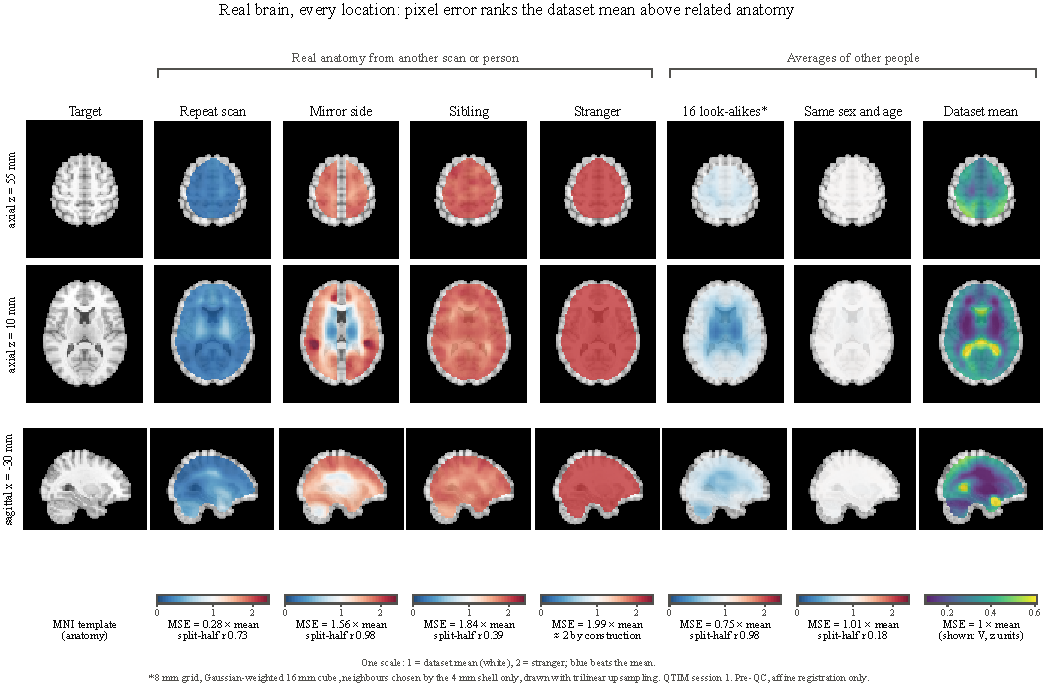
\includegraphics[width=\textwidth]{fig/brain_gaussian_maps.pdf}
\caption{\textbf{Saved provisional Gaussian brain maps.}
Population-template anatomy underlies aggregated donor-error maps.
The source remains pre-QC with affine registration.
Displayed local errors use the Gaussian amendments; the coarser look-alike grid is interpolated for display.
The source image title is a descriptive pixel-error statement, not a validated biological identity conclusion.
Source figure: \src{results/figures/fig_ladder_maps_common.pdf}; quantitative sources are the brain map and map-grid JSONs.}
\label{fig:s-brain}
\end{figure*}


\section{Directional tests and uncertainty}
The recorded tests have explicit reference candidates.
T1 compares repeat with dataset mean; T2 compares repeat with its attenuated version; T3a compares repeat with incorrect detail; T3b compares repeat with white noise.
The paired independent unit is a family for QTIM and a person for iris.
The fundus v1 panel uses a repeat reference for GRAPE and a fellow-eye reference for PAPILA; PAPILA has no T1 comparison.
The corresponding source protocol specifies its Holm family, and unavailable comparisons retain their status rather than becoming successful tests.

\begin{table*}[t]
\centering
\caption{\textbf{Recorded brain directional tests, provisional.}
Each cell reports the source decision and Holm-adjusted probability.
The test is one-sided in favor of the repeat.
Not establishing T2 is not an equivalence result.
Residual correlation versus the exact mean has no eligible T1 pair.
Source: \src{results/donor_ladder_brain_metrics.json}, random-region LR view.}
\small
\begin{tabular}{@{}lcccc@{}}
\toprule
Metric & T1 & T2 & T3a & T3b \\
\midrule
MSE & pass (6.6e-06)\statuspre & not established (1)\statuspre & pass (6.6e-06)\statuspre & pass (6.6e-06)\statuspre \\
SSIM & pass (6.6e-06)\statuspre & not established (1)\statuspre & pass (6.6e-06)\statuspre & pass (6.6e-06)\statuspre \\
Residual correlation & \notrun & not established (1)\statuspre & pass (6.6e-06)\statuspre & pass (6.6e-06)\statuspre \\
TM-like & pass (6.6e-06)\statuspre & not established (1)\statuspre & pass (6.6e-06)\statuspre & pass (6.6e-06)\statuspre \\
lDDT-like, repeat tolerance & pass (6.6e-06)\statuspre & not established (1)\statuspre & pass (6.6e-06)\statuspre & pass (6.6e-06)\statuspre \\
\bottomrule

\end{tabular}
\end{table*}

Source intervals resample independent clusters and, where specified, positions.
The cluster-only interval retained in the source answers a different uncertainty question from the two-way interval.
Neither interval repairs registration bias or an incorrect identity definition.
No new confidence interval or hypothesis test is recomputed from the published aggregate summaries.

\section{Available metric registry}
The fixed registry distinguishes computed, blocked and unavailable metrics before a ranking is interpreted.
The following table compares the completed fundus v1 registry with the accessible iris P2 registry.
A later unblocking amendment does not change these historical run statuses.
The main brain table uses its own tier-1 definitions and resampling scheme.

{\small
\begin{longtable}{@{}lll@{}}
\caption{Metric availability in the frozen sources.
Sources: \src{results/fundus_ladder_metrics.json} at the bilateral snapshot and \src{results/iris_ladder_metrics.json}.}\\
\toprule
Metric & Fundus v1 & Iris P2 \\
\midrule
\endfirsthead
\toprule
Metric & Fundus v1 & Iris P2 \\
\midrule
\endhead
mse & computed & computed \\
rmse & computed & computed \\
psnr & computed & computed \\
mae & computed & computed \\
ssim & computed & computed \\
ms\_ssim & computed & computed \\
lpips & blocked & blocked \\
acc\_dataset & computed & computed \\
acc\_matched & computed & blocked \\
amplitude\_dataset & computed & computed \\
amplitude\_matched & computed & blocked \\
lddt & computed & computed \\
intensity\_persistence & computed & computed \\
betti\_matching\_matched & blocked & blocked \\
betti\_matching\_unmatched & blocked & blocked \\
id\_angle & blocked & blocked \\
id\_norm & blocked & blocked \\
id\_pfe & blocked & blocked \\
id\_plda & blocked & blocked \\
latent\_pullback & blocked & blocked \\
latent\_fisher\_rao & blocked & blocked \\
latent\_lddmm & blocked & blocked \\
plausibility & blocked & blocked \\
fid & blocked & blocked \\
fwd & blocked & blocked \\
topology\_distance & blocked & blocked \\
\bottomrule

\end{longtable}
}

\clearpage
\section{CARE aggregation audit as related evidence}
The repository also contains a separate reproduction attempt on the released CARE scores~\cite{care2025}.
Its current iteration records the status of each published median/quartile comparison under the frozen aggregation rule.
This is a consistency audit of released scores, not generation of reconstructed CT or a rerun of the image-level segmenter.
An aggregation mismatch does not refute the anatomical benefit of the reconstruction method.
Coverage failures and non-finite values remain distinct from numeric disagreement.

\begin{table}[htbp]
\centering
\caption{Saved CARE iteration-2 comparison statuses, counted directly from the source rows.
Source: \src{results/care_iteration2.json}.
The status names refer to the recorded numerical comparison, not the validity of CARE's broader scientific claims.}
\begin{tabular}{@{}lr@{}}
\toprule
Recorded comparison status & Count \\
\midrule
Within the recorded rounding tolerance & 36 \\
Outside that tolerance & 63 \\
Blocked by coverage & 8 \\
No finite available comparison & 1 \\
\bottomrule

\end{tabular}
\end{table}

\section{Correlation and historical size sensitivity}
The saved correlation analysis groups distances by their rung-order dependence within target, position and side.
Strong agreement among monotone variants is not independent confirmation of identity sensitivity.
The saved size/shell sweep varies older window and context choices; it is not the completed object-relative sweep specified by the latest amendment.
Both figures remain provisional and retain the source protocol's interpretation.

\clearpage
\begin{figure}[p]
\centering
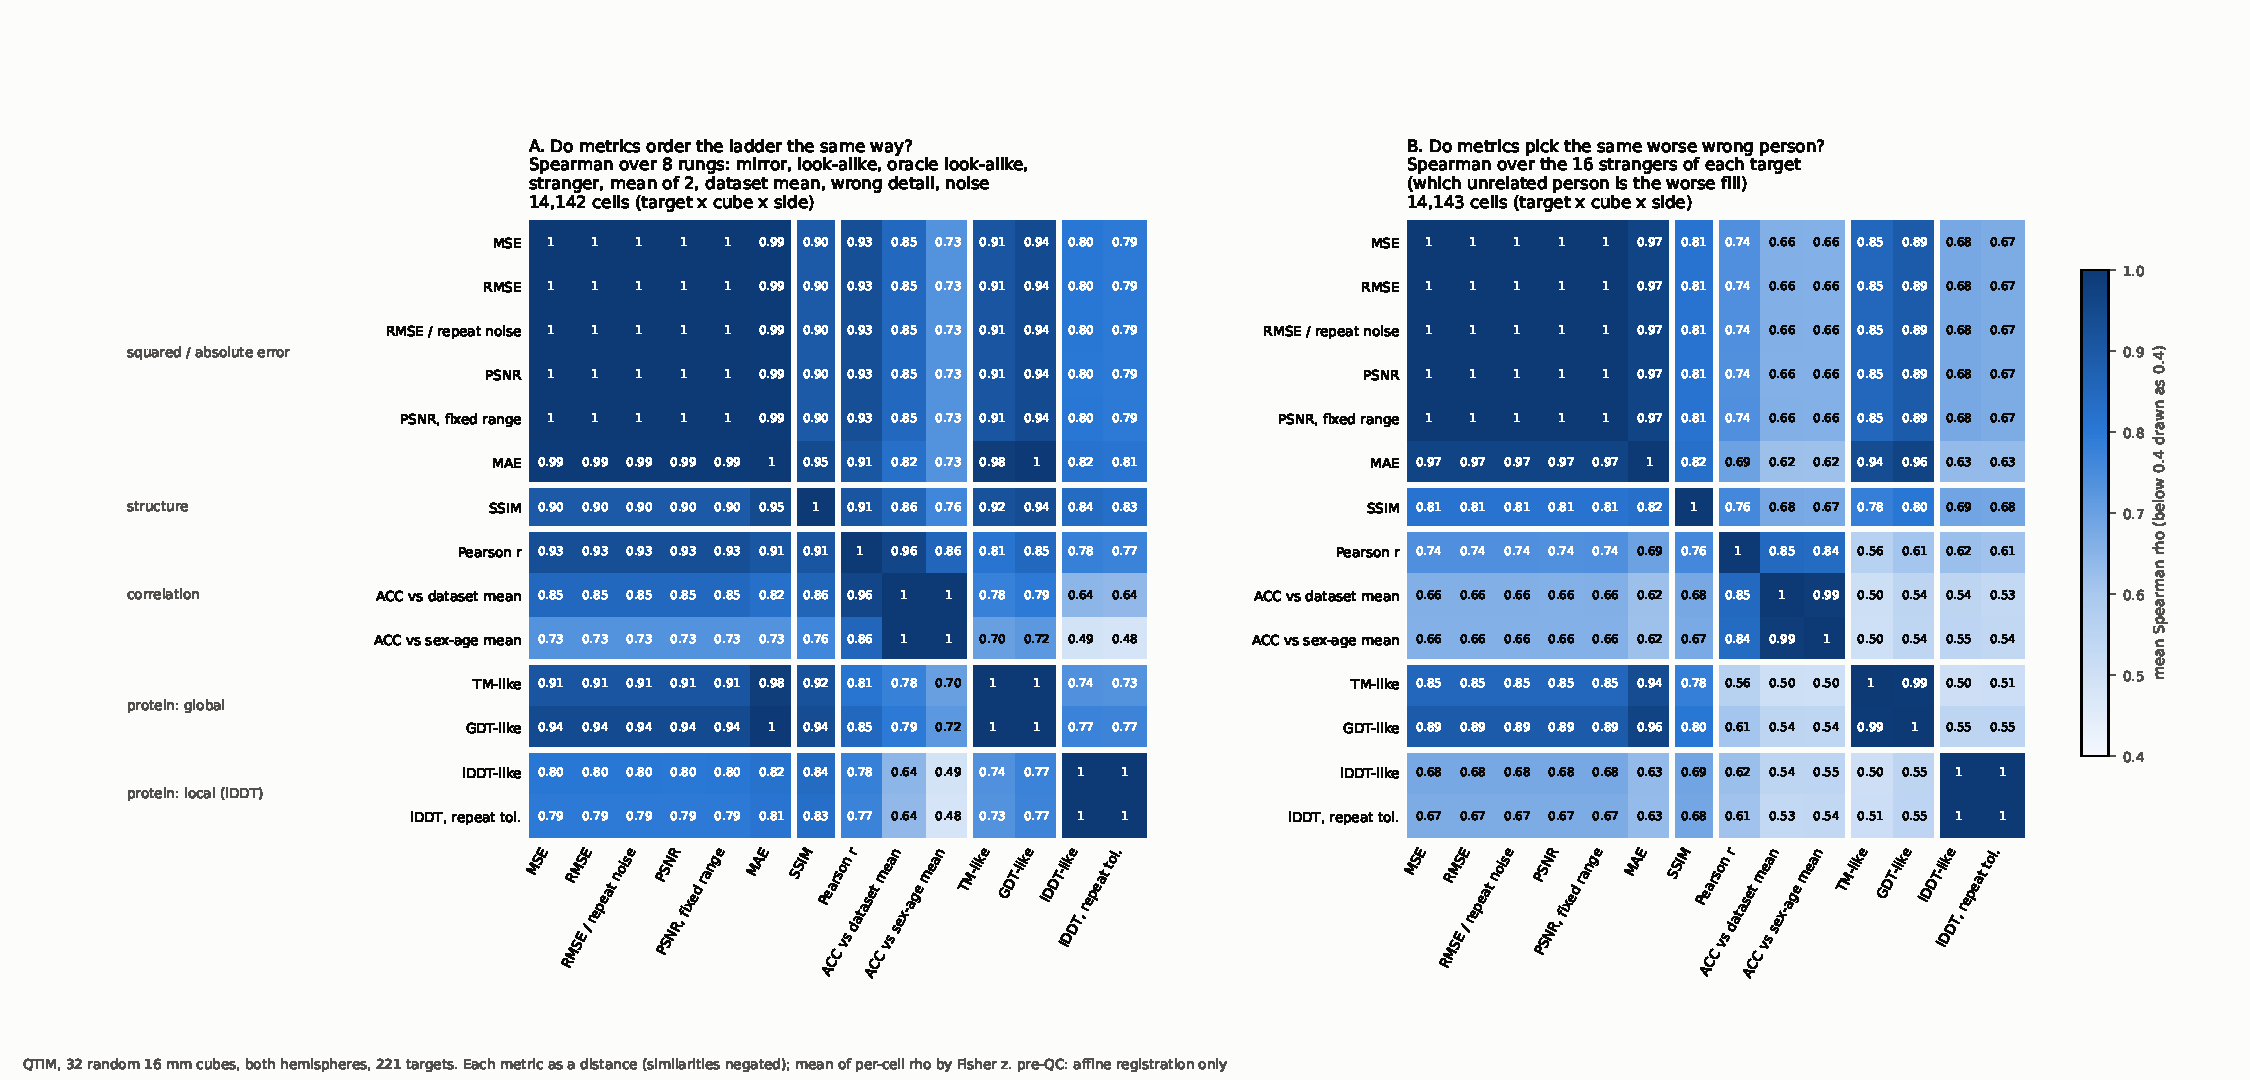
\includegraphics[width=.9\textwidth,height=.72\textheight,keepaspectratio]{fig/metric_correlations.pdf}
\caption{Saved provisional metric-dependence analysis.
Source: \src{results/figures/fig_metrics_correlation.pdf}, with \src{results/donor_ladder_metrics_correlation.json}.
This is descriptive dependence among measures, not a learned fusion or a ranking of validated identity metrics.}
\end{figure}

\clearpage
\begin{figure}[p]
\centering
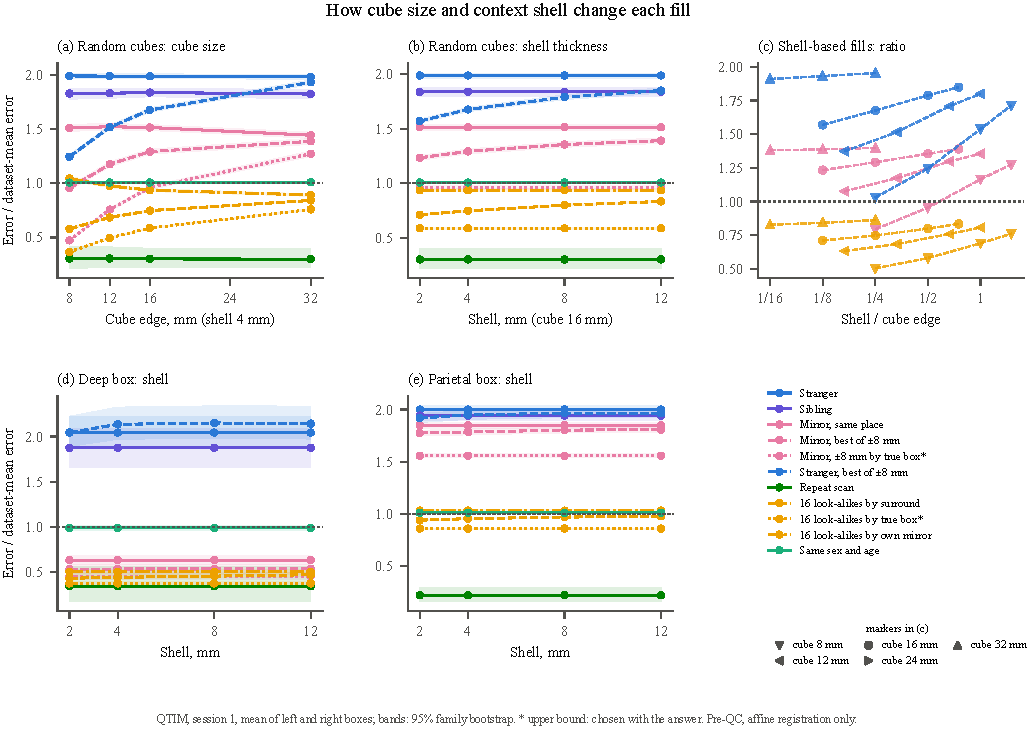
\includegraphics[width=.95\textwidth,height=.72\textheight,keepaspectratio]{fig/size_shell_sensitivity.pdf}
\caption{Saved provisional window/context sensitivity from the earlier sweep.
Source: \src{results/figures/fig_size_shell_dependence.pdf}, with \src{results/donor_ladder_brain_size.json}.
The figure does not establish completion of the latest object-relative metric-panel sweep.}
\end{figure}
\clearpage

\section{Full selected brain profiles}
Table~\ref{tab:s-brain-full} preserves endpoint-specific target and family counts for the selected rungs across all available tier-1 distances.
These are provisional random-region LR values and do not replace a post-registration panel.

{\small
\begin{longtable}{@{}llcrr@{}}
\caption{Selected saved brain $R_{\rm rep}$ profiles and 95\% intervals.
Source: \src{results/donor_ladder_brain_metrics.json}.}
\label{tab:s-brain-full}\\
\toprule
Metric & Rung & $R_{\rm rep}$ & Targets & Families \\
\midrule
\endfirsthead
\toprule
Metric & Rung & $R_{\rm rep}$ & Targets & Families \\
\midrule
\endhead
mse & dataset\_mean & \shortstack{0.413\statuspre\\{\scriptsize [0.367, 0.443]}} & 221 & 168 \\
mse & mirror & \shortstack{0.717\statuspre\\{\scriptsize [0.622, 0.792]}} & 221 & 168 \\
mse & repeat & \shortstack{0.000\statuspre\\{\scriptsize [0.000, 0.000]}} & 23 & 23 \\
mse & shrink\_repeat & \shortstack{-0.014\statuspre\\{\scriptsize [-0.028, -0.004]}} & 23 & 23 \\
mse & wrong\_detail & \shortstack{1.006\statuspre\\{\scriptsize [0.992, 1.020]}} & 221 & 168 \\
mse & noise & \shortstack{0.921\statuspre\\{\scriptsize [0.893, 0.944]}} & 221 & 168 \\
rmse & dataset\_mean & \shortstack{0.538\statuspre\\{\scriptsize [0.488, 0.573]}} & 221 & 168 \\
rmse & mirror & \shortstack{0.766\statuspre\\{\scriptsize [0.682, 0.830]}} & 221 & 168 \\
rmse & repeat & \shortstack{0.000\statuspre\\{\scriptsize [0.000, 0.000]}} & 23 & 23 \\
rmse & shrink\_repeat & \shortstack{-0.015\statuspre\\{\scriptsize [-0.031, -0.002]}} & 23 & 23 \\
rmse & wrong\_detail & \shortstack{1.001\statuspre\\{\scriptsize [0.993, 1.010]}} & 221 & 168 \\
rmse & noise & \shortstack{0.943\statuspre\\{\scriptsize [0.924, 0.958]}} & 221 & 168 \\
mae & dataset\_mean & \shortstack{0.554\statuspre\\{\scriptsize [0.495, 0.595]}} & 221 & 168 \\
mae & mirror & \shortstack{0.702\statuspre\\{\scriptsize [0.593, 0.784]}} & 221 & 168 \\
mae & repeat & \shortstack{0.000\statuspre\\{\scriptsize [0.000, 0.000]}} & 23 & 23 \\
mae & shrink\_repeat & \shortstack{-0.014\statuspre\\{\scriptsize [-0.033, 0.000]}} & 23 & 23 \\
mae & wrong\_detail & \shortstack{0.997\statuspre\\{\scriptsize [0.987, 1.007]}} & 221 & 168 \\
mae & noise & \shortstack{0.997\statuspre\\{\scriptsize [0.970, 1.031]}} & 221 & 168 \\
psnr & dataset\_mean & \shortstack{0.664\statuspre\\{\scriptsize [0.611, 0.702]}} & 221 & 168 \\
psnr & mirror & \shortstack{0.815\statuspre\\{\scriptsize [0.744, 0.870]}} & 221 & 168 \\
psnr & repeat & \shortstack{0.000\statuspre\\{\scriptsize [0.000, 0.000]}} & 23 & 23 \\
psnr & shrink\_repeat & \shortstack{-0.014\statuspre\\{\scriptsize [-0.036, 0.004]}} & 23 & 23 \\
psnr & wrong\_detail & \shortstack{1.000\statuspre\\{\scriptsize [0.994, 1.005]}} & 221 & 168 \\
psnr & noise & \shortstack{0.963\statuspre\\{\scriptsize [0.950, 0.973]}} & 221 & 168 \\
psnr\_fixed & dataset\_mean & \shortstack{0.666\statuspre\\{\scriptsize [0.613, 0.704]}} & 221 & 168 \\
psnr\_fixed & mirror & \shortstack{0.816\statuspre\\{\scriptsize [0.744, 0.872]}} & 221 & 168 \\
psnr\_fixed & repeat & \shortstack{0.000\statuspre\\{\scriptsize [0.000, 0.000]}} & 23 & 23 \\
psnr\_fixed & shrink\_repeat & \shortstack{-0.014\statuspre\\{\scriptsize [-0.035, 0.004]}} & 23 & 23 \\
psnr\_fixed & wrong\_detail & \shortstack{1.000\statuspre\\{\scriptsize [0.994, 1.005]}} & 221 & 168 \\
psnr\_fixed & noise & \shortstack{0.963\statuspre\\{\scriptsize [0.950, 0.974]}} & 221 & 168 \\
ssim & dataset\_mean & \shortstack{0.738\statuspre\\{\scriptsize [0.680, 0.784]}} & 221 & 168 \\
ssim & mirror & \shortstack{0.823\statuspre\\{\scriptsize [0.755, 0.873]}} & 221 & 168 \\
ssim & repeat & \shortstack{0.000\statuspre\\{\scriptsize [0.000, 0.000]}} & 23 & 23 \\
ssim & shrink\_repeat & \shortstack{0.001\statuspre\\{\scriptsize [-0.015, 0.016]}} & 23 & 23 \\
ssim & wrong\_detail & \shortstack{1.023\statuspre\\{\scriptsize [1.014, 1.036]}} & 221 & 168 \\
ssim & noise & \shortstack{1.132\statuspre\\{\scriptsize [1.088, 1.194]}} & 221 & 168 \\
pearson & dataset\_mean & \shortstack{0.581\statuspre\\{\scriptsize [0.547, 0.610]}} & 221 & 168 \\
pearson & mirror & \shortstack{0.817\statuspre\\{\scriptsize [0.757, 0.869]}} & 221 & 168 \\
pearson & repeat & \shortstack{0.000\statuspre\\{\scriptsize [0.000, 0.000]}} & 23 & 23 \\
pearson & shrink\_repeat & \shortstack{-0.005\statuspre\\{\scriptsize [-0.009, -0.003]}} & 23 & 23 \\
pearson & wrong\_detail & \shortstack{1.013\statuspre\\{\scriptsize [1.002, 1.026]}} & 221 & 168 \\
pearson & noise & \shortstack{0.989\statuspre\\{\scriptsize [0.985, 0.994]}} & 221 & 168 \\
acc\_dataset & dataset\_mean & \textit{undefined} & \textit{undefined} & \textit{undefined} \\
acc\_dataset & mirror & \shortstack{0.752\statuspre\\{\scriptsize [0.688, 0.808]}} & 221 & 168 \\
acc\_dataset & repeat & \shortstack{0.000\statuspre\\{\scriptsize [0.000, 0.000]}} & 23 & 23 \\
acc\_dataset & shrink\_repeat & \shortstack{-0.000\statuspre\\{\scriptsize [-0.000, 0.000]}} & 23 & 23 \\
acc\_dataset & wrong\_detail & \shortstack{1.003\statuspre\\{\scriptsize [0.996, 1.009]}} & 221 & 168 \\
acc\_dataset & noise & \shortstack{1.003\statuspre\\{\scriptsize [1.000, 1.006]}} & 221 & 168 \\
acc\_cohort & dataset\_mean & \shortstack{0.893\statuspre\\{\scriptsize [0.883, 0.903]}} & 221 & 168 \\
acc\_cohort & mirror & \shortstack{0.755\statuspre\\{\scriptsize [0.691, 0.811]}} & 221 & 168 \\
acc\_cohort & repeat & \shortstack{0.000\statuspre\\{\scriptsize [0.000, 0.000]}} & 23 & 23 \\
acc\_cohort & shrink\_repeat & \shortstack{-0.000\statuspre\\{\scriptsize [-0.000, 0.000]}} & 23 & 23 \\
acc\_cohort & wrong\_detail & \shortstack{1.003\statuspre\\{\scriptsize [0.995, 1.009]}} & 221 & 168 \\
acc\_cohort & noise & \shortstack{1.001\statuspre\\{\scriptsize [0.999, 1.004]}} & 221 & 168 \\
lddt & dataset\_mean & \shortstack{0.375\statuspre\\{\scriptsize [0.301, 0.434]}} & 221 & 168 \\
lddt & mirror & \shortstack{0.889\statuspre\\{\scriptsize [0.842, 0.925]}} & 221 & 168 \\
lddt & repeat & \shortstack{0.000\statuspre\\{\scriptsize [0.000, 0.000]}} & 23 & 23 \\
lddt & shrink\_repeat & \shortstack{-0.069\statuspre\\{\scriptsize [-0.088, -0.053]}} & 23 & 23 \\
lddt & wrong\_detail & \shortstack{1.056\statuspre\\{\scriptsize [1.034, 1.086]}} & 221 & 168 \\
lddt & noise & \shortstack{2.159\statuspre\\{\scriptsize [2.013, 2.347]}} & 221 & 168 \\
tm\_like & dataset\_mean & \shortstack{0.723\statuspre\\{\scriptsize [0.642, 0.778]}} & 221 & 168 \\
tm\_like & mirror & \shortstack{0.667\statuspre\\{\scriptsize [0.530, 0.761]}} & 221 & 168 \\
tm\_like & repeat & \shortstack{0.000\statuspre\\{\scriptsize [0.000, 0.000]}} & 23 & 23 \\
tm\_like & shrink\_repeat & \shortstack{-0.013\statuspre\\{\scriptsize [-0.041, 0.008]}} & 23 & 23 \\
tm\_like & wrong\_detail & \shortstack{0.997\statuspre\\{\scriptsize [0.987, 1.007]}} & 221 & 168 \\
tm\_like & noise & \shortstack{1.075\statuspre\\{\scriptsize [1.041, 1.121]}} & 221 & 168 \\
gdt\_like & dataset\_mean & \shortstack{0.676\statuspre\\{\scriptsize [0.601, 0.727]}} & 221 & 168 \\
gdt\_like & mirror & \shortstack{0.680\statuspre\\{\scriptsize [0.551, 0.771]}} & 221 & 168 \\
gdt\_like & repeat & \shortstack{0.000\statuspre\\{\scriptsize [0.000, 0.000]}} & 23 & 23 \\
gdt\_like & shrink\_repeat & \shortstack{-0.014\statuspre\\{\scriptsize [-0.039, 0.006]}} & 23 & 23 \\
gdt\_like & wrong\_detail & \shortstack{0.996\statuspre\\{\scriptsize [0.985, 1.005]}} & 221 & 168 \\
gdt\_like & noise & \shortstack{1.054\statuspre\\{\scriptsize [1.023, 1.095]}} & 221 & 168 \\
lddt\_rep & dataset\_mean & \shortstack{0.355\statuspre\\{\scriptsize [0.254, 0.430]}} & 221 & 168 \\
lddt\_rep & mirror & \shortstack{0.890\statuspre\\{\scriptsize [0.843, 0.925]}} & 221 & 168 \\
lddt\_rep & repeat & \shortstack{0.000\statuspre\\{\scriptsize [0.000, 0.000]}} & 23 & 23 \\
lddt\_rep & shrink\_repeat & \shortstack{-0.084\statuspre\\{\scriptsize [-0.108, -0.065]}} & 23 & 23 \\
lddt\_rep & wrong\_detail & \shortstack{1.050\statuspre\\{\scriptsize [1.030, 1.080]}} & 221 & 168 \\
lddt\_rep & noise & \shortstack{2.073\statuspre\\{\scriptsize [1.924, 2.273]}} & 221 & 168 \\
rmse\_rep & dataset\_mean & \shortstack{0.539\statuspre\\{\scriptsize [0.487, 0.576]}} & 221 & 168 \\
rmse\_rep & mirror & \shortstack{0.766\statuspre\\{\scriptsize [0.681, 0.833]}} & 221 & 168 \\
rmse\_rep & repeat & \shortstack{0.000\statuspre\\{\scriptsize [0.000, 0.000]}} & 23 & 23 \\
rmse\_rep & shrink\_repeat & \shortstack{-0.014\statuspre\\{\scriptsize [-0.030, -0.001]}} & 23 & 23 \\
rmse\_rep & wrong\_detail & \shortstack{1.002\statuspre\\{\scriptsize [0.994, 1.010]}} & 221 & 168 \\
rmse\_rep & noise & \shortstack{0.944\statuspre\\{\scriptsize [0.924, 0.959]}} & 221 & 168 \\
\bottomrule

\end{longtable}
}

\section{Advanced metrics and unavailable endpoints}
The iris extension prespecifies LPIPS~\cite{zhang2018lpips}, Betti matching~\cite{betti2023}, and distribution-level FID/FWD comparisons~\cite{heusel2017fid,fwd2025}.
These measurements operate at different levels.
A set-level distribution distance cannot be treated as a per-eye identity distance, and Betti matching on intensity filtrations is an adaptation from its segmentation setting.
The protocol records hypotheses about attenuation, realism and repeat--look-alike--stranger order.
Those expectations must be tested rather than imposed as the order of a plot.

The workstation handoff reports that the full iris P3 run finished, with a Betti-related H4 failure and support for H5 and H6.
Its numerical aggregate outputs are absent from the accessible Git snapshot.
This assembly therefore retains that report as a pending source-integration item and makes no numerical P3 claim.
It must not be replaced by P2 or by the older classical-code pilot.
Brain-ID embeddings, complete model-level inpainting comparisons, and the latest object-relative size sweep likewise require their own completed evidence before being claimed.

\section{Cross-anatomy metric profiles}
The source-derived profile figure retains its distinct anchors and unresolved MRI status.
Its role is to compare measured responses to controls, not to select a competition metric by averaging across anatomical domains.

\begin{figure}[htbp]
\centering
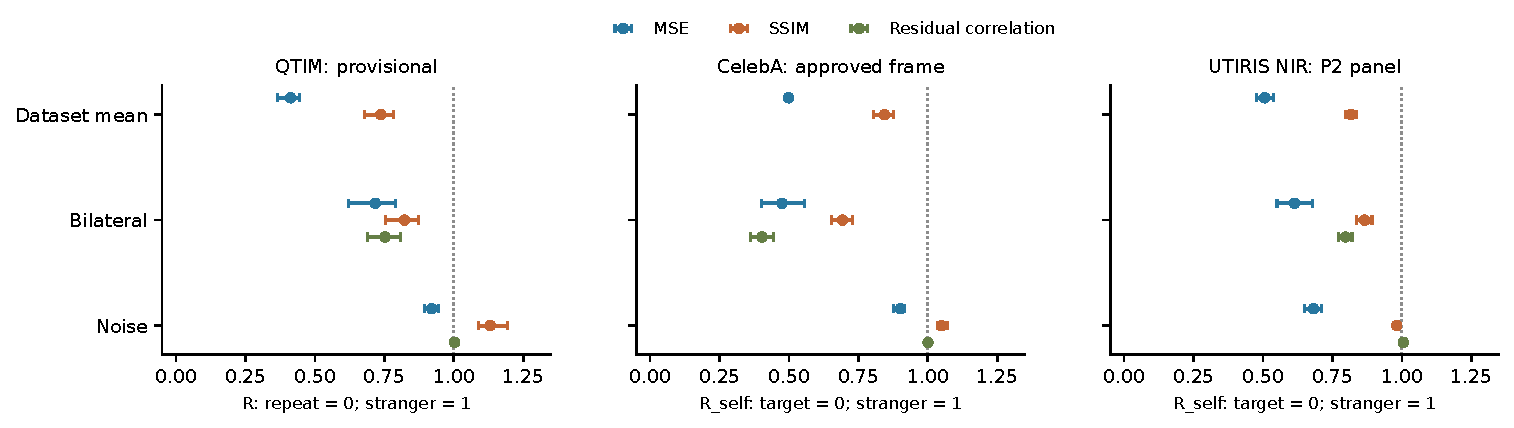
\includegraphics[width=\textwidth]{fig/audit_profiles.pdf}
\caption{Mean, bilateral and noise controls show different metric profiles.
QTIM uses the repeat anchor and remains provisional; CelebA and UTIRIS use self anchors.
The absent residual-correlation point at the mean is undefined.
Sources: the saved brain, face and iris metric-panel JSONs; generated by the paper preparation script.}
\end{figure}

\section{Reproducibility and outstanding author inputs}
The manuscript preparation is independent of historical absolute data paths and operates from the repository root.
The human-image experiment pipelines retain source-specific model and data requirements, and their presence in Git does not establish execution on this host.
The base face pipeline, latest fundus metric run, and full iris P3 require safe exports from their owners.
The atlas supplied here replaces the stale brain row with saved Gaussian aggregate panels and records every assembly transformation.
It does not recompute the maps from the private data, and its scalar annotations summarize pooled source errors rather than only the displayed axial slice.

The related ISBI source is preserved.
Publication overlap, dataset-specific ethics statements, portal requirements, and final author approval remain separate from successful typesetting.
No push is performed before the author reviews the rendered PDFs.


\end{document}
